% ----------------------------------------------------------
% Metodologia
% ----------------------------------------------------------
\chapter{Metodologia}
\label{cha:metodologia}

Para o levantamento e definição do escopo dos requisitos do sistema, foi empregado o método Joint Application Design (JAD). Este modelo de levantamento de requisitos envolve os usuários finais e a equipe de desenvolvimento, garantindo que ambos compreendam a finalidade e o potencial que o software a ser desenvolvido trará \mbox{\cite{b:escolpo_projeto_2015}.} Através do conhecimento multidisciplinar, busca-se identificar as necessidades e estabelecer metas claras para o desenvolvimento do sistema, em conjunto com a metodologia SCRUM, que organiza as atividades em sprints para um desenvolvimento mais eficaz \mbox{\cite{b:scrum2015}.}

A esquematização para o desenvolvimento de um sistema é fundamental. Neste trabalho, foi adotado a abordagem de sprints para o desenvolvimento do sistema. A Figura \ref{fig:banco_dados} é analisada por meio dessa metodologia SCRUM, de modo.

\begin{figure}[htb!]
    \centering
    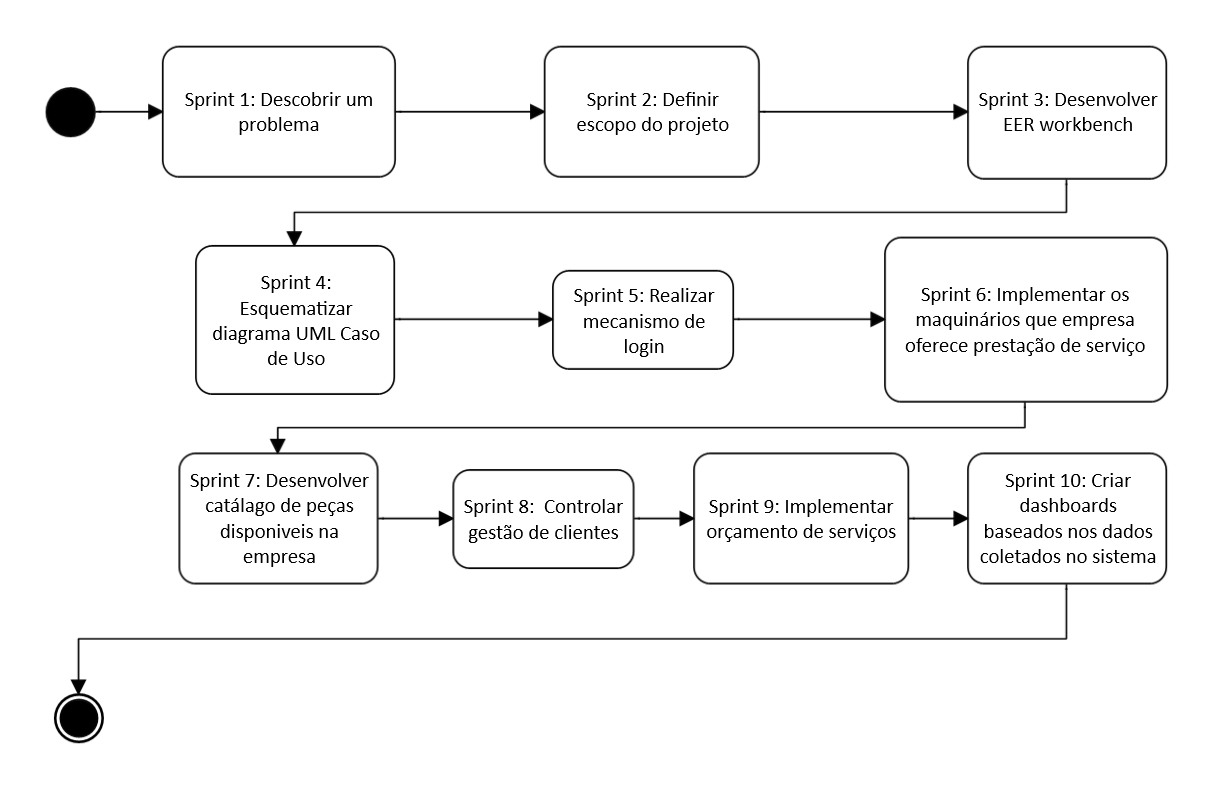
\includegraphics[width=0.75\linewidth]{figs/sprint_novo_modelo.png}
    \caption{Sprints implementação do sistema V Tornos}
    \label{fig:sprints}
\end{figure}

\section{Sprint 1: Descobrir um problema}
\label{sec:descobrir_problema}

O sprint 1 é fundamental para a definição do projeto, permitindo identificar claramente o motivo pelo qual determinado software ou ação está sendo desenvolvido. Nesse contexto, alguns pensadores destacam a importância do "telos", ou finalidade, na filosofia. Compreender esse propósito possibilita a análise do cenário e a busca por medidas que promovam a evolução contínua.

Com o surgimento do Minimum Viable Product (MVP), que tem suas raízes na manufatura enxuta, originada pelo modelo Toyotista. O objetivo do MVP é viabilizar a aceitação de um produto com as características essenciais, permitindo que os desenvolvedores realizem ajustes e evoluções com base no feedback do mercado. Dessa forma, é possível economizar esforço e recursos, evitando o investimentos de tempo e capital em características que possam não ter aceitação pelo público \mbox{\cite{a:mvp_2023}.}

\section{Sprint 2: Definir escolpo do projeto}
\label{sec:definir_escolpo}

Com o auxílio do Sprint 1, são definidas a ideia principal e a utilização do MVP. O Sprint 2 proporciona o contexto apropriado para esclarecer seu propósito, os problemas que busca resolver e as características específicas que aprimorarão a experiência do usuário. No sistema V Tornos, o objetivo é desenvolver uma solução inovadora para a gestão de dados no fluxo de orçamento e serviços, garantindo que as novas etapas do software estejam sempre alinhadas a esse propósito.

\section{Sprint 3: Desenvolver EER Workbench}
\label{sec:desenvolver_eer}

Antes de escolher o ambiente de desenvolvimento e o tipo de banco de dados, é fundamental identificar os dados que serão persistidos. Após essa etapa, é importante decidir entre um banco de dados relacional ou não relacional, levando em conta a possibilidade de migração do sistema para outra plataforma no futuro. Dessa forma, os dados permanecerão acessíveis, independentemente do ambiente escolhido. A Figura \ref{fig:banco_dados} ilustra os dados que o sistema manejará por meio do CodeIgniter.

\begin{figure}[ht!]
\centering
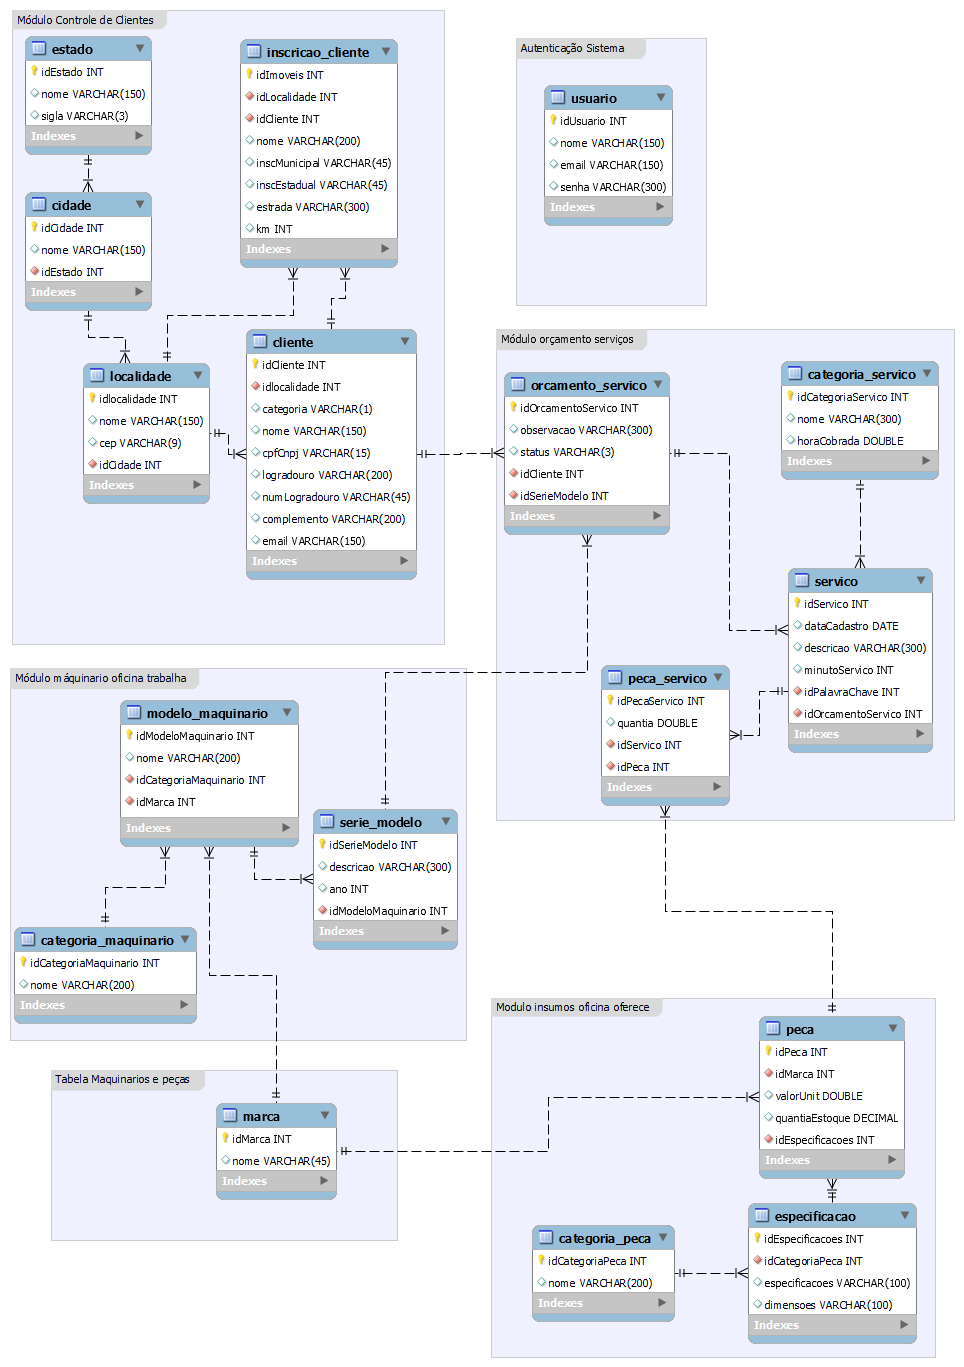
\includegraphics[width=0.76\linewidth]{figs/base_dados_firma.png}
\caption{Estrutura do banco de dados V Tornos}
\label{fig:banco_dados}
\end{figure}

\section{Sprint 4: Esquematizar diagrama UML Caso de uso}
\label{sec:esquematizar_uml}

A Figura \ref{fig:caso_uso} apresenta um modelo de caso de uso que descreve as ações esperadas dos usuários do sistema, evidenciando que haverá um único nível de acesso. Dessa forma, o ator necessitará ter acesso ao sistema para realizar as atividades definidas. O modelo de caso de uso busca ilustrar e identificar as funcionalidades do sistema através de uma abordagem visual simplificada, sem especificar a estrutura de implementação. Essa metodologia facilita a análise objetiva do sistema, apresentando um padrão de fácil compreensão e destacando as interações entre o sistema e o ator.

\begin{figure}[h!]
    \centering
    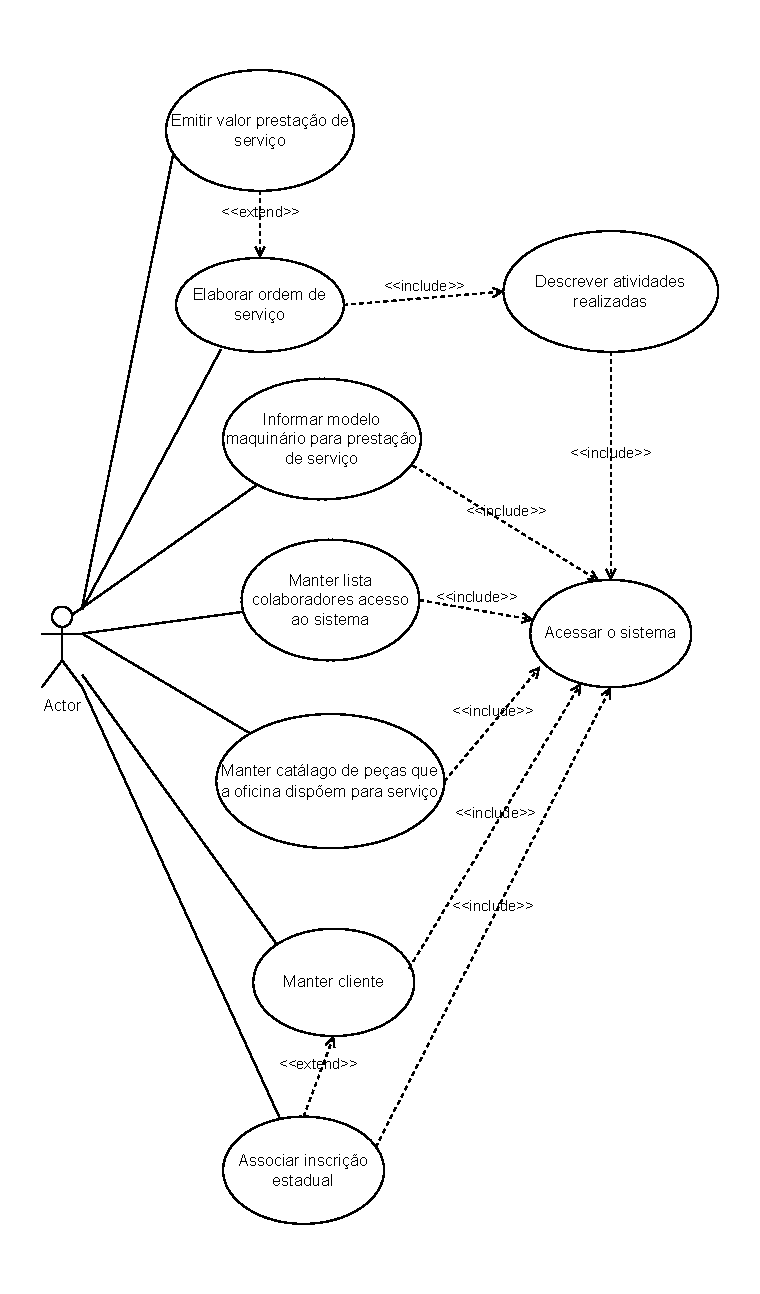
\includegraphics[width=0.50\linewidth]{figs/TCC_Caso_de_Uso.pdf}
    \caption{Diagrama de caso de uso V Tornos}
    \label{fig:caso_uso}
\end{figure}

\section{Sprint 5: Realizar mecanismo de login}
\label{sec:Sprint_login}

Com o objetivo de garantir que as páginas sejam acessíveis apenas a usuários autorizados, o sistema V Tornos implementa um controle de acesso por meio da classe Filter, que pode ser desenvolvida utilizando o Spark. Ao criar um Filter, o CodeIgniter disponibiliza dois métodos: before e after. Para assegurar a segurança das páginas, a implementação ocorre no método before, onde será realizada uma verificação para determinar se a visualização de uma determinada página pode ser permitida o acesso.

\section{Sprint 6: Implementar os maquinários que empresa oferece prestação de serviço}
\label{label:maquinarios}

A seguinte etapa, visa organizar o desenvolvimento de maquinários para a prestação de serviços. Sendo as tabelas ``marca'' e ``maquinário'' tabelas auxiliares para o ``modelo''. Além disso, a tabela "série" estabelecerá um relacionamento de muitos para um (nx1) com a tabela ``orçamento''.

\section{Sprint 7: Desenvolver catálago de peças disponíveis na empresa}
\label{sec:pecas}

Para otimizar a entrega do maquinário, a empresa mantém um estoque de peças de uso geral. Esse sistema de estoque é composto por quatro tabelas, sendo a tabela "marca" uma das principais, pois também se conecta à tabela de maquinários. Isso ocorre porque existem marcas que fabricam suas próprias peças, além de haver no mercado peças paralelas a um preço mais baixo. A decisão sobre qual opção escolher fica a critério do cliente.

\section{Sprint 8: Controlar gestão de clientes}
\label{sec:clientes}

Para gerenciar de maneira eficaz os dados dos clientes, o sistema é composto por cinco tabelas. As duas tabelas principais são ``cliente'' e ``inscrição'' refere as inscrições municipais, estaduais e o nome do imóvel. Para facilitar a localização dessas informações, existe um conjunto hierárquico de tabelas que inclui "estado", "cidade" e "localidade", as quais indicarão o local do imóvel. Esse conjunto também será utilizado para a emissão da Nota Fiscal de Serviço Eletrônica, permitindo a realização das devidas cobranças de forma eficiente.

\section{Sprint 9:Implementar gerenciamento de orçamento e serviços}
\label{sec:orcamentos_servicos}

Os sprints anteriores têm como objetivo dar suporte ao desenvolvimento desta etapa, pois é necessário identificar quais maquinários a empresa oferece serviços, além de disponibilizar um catálogo de peças para substituição nos equipamentos. Por fim, visa atender aos clientes que buscam o V Tornos para resolver situações específicas relacionadas aos maquinários. Assim, este sprint se concentra em quatro tabelas, que contêm relações conforme mencionado.

A tabela "categoria serviço" tem como finalidade manter os tipos de usinamento ou atividades, conforme ilustrado na Figura \ref{fig:tipo_usinagem}, juntamente com o respectivo valor por hora de serviço. A tabela "peça serviço" informa a quantidade de peças que serão utilizadas para cada solução, possibilitando uma estimativa precisa do valor final, já incluindo as peças. A tabela "orçamento" especifica qual maquinário receberá manutenção por parte do respectivo cliente. Por fim, a tabela "serviço" descreve as atividades, que podem constituir um conjunto de ações documentadas para suprir a reparação de componentes do maquinário.

\section{Sprint 10: Criar dashboards baseados nos dados coletados no sistema}
\label{sec:dashboards}

O sprint 10 tem como objetivo desenvolver um dashboard para o sistema, que permitirá a geração de relatórios em forma de gráficos. Esses relatórios mostrarão as atividades mais rotineiras e identificarão quais maquinários estão frequentemente presentes na operação. Com essa funcionalidade, será possível obter uma compreensão mais profunda sobre quais clientes são fidelizados pela V Tornos, oferecendo uma visão abrangente do desempenho e das relações comerciais.

\section{Uso da inteligência artificial}
\label{sec:IA}

Atualmente, existem tecnologias que possibilitam a criação de modelos artificiais que se assemelham à perspectiva da inteligência humana, uma ideia inicialmente proposta por Alan Turing na reflexão se ``Podem as máquinas pensar?", atualmente denominada como Teste de Turing Ideal (TTI) \cite{b:AI_Alan_Turing_2023}. Nesse contexto, a OpenAI foi desenvolvida a partir de um grupo de acionistas, incluindo empreendedores de destaque como Elon Musk e Sam Altman. Para que as empresas possam explorar melhor as informações, o Chat \textit{Generative Pre-trained Transformer} (GPT) se apresenta como uma ferramenta eficaz para indivíduos e organizações \mbox{\cite{a:chat_gpt_2023}.}

Quando utilizada com bom senso e responsabilidade, a inteligência artificial pode oferecer grandes benefícios à sociedade e nas empresas. Ela ajuda a organizar e aprimorar a busca por conhecimento, além de simplificar várias atividades. No entanto, é essencial que o usuário tenha clareza sobre o que busca e consiga distinguir entre falácias e verdades no tema em que deseja se aprofundar.

Além disso, em termos de ética e moral, é importante mencionar que este trabalho recebeu contribuições do uso do Chat GPT para auxiliar na estruturação dos tópicos. O objetivo foi buscar um modelo de fácil leitura e didática para os conhecimentos importantes para o entendimento da proposta, com "telos" como abordagem central e melhoria na documentação de serviços artesanais na fabricação ou reparação de peças para o meio agrícola e pecuária.
